\chapter{Analysis techniques}

\intro{This chapter introduces the necessary toolset to perform the analyses within this thesis. It is organized to follow the common steps of the analyses. First, the generation of simulated events is introduced. Then, details of the top quark reconstruction, the employed multivariate analysis technique, and the template fit is given which are used to estimate the amount of single top quark events within the recorded data. Lastly, the partonic and fiducial objects are defined to which the observed data is unfolded to for comparison with theoretical predictions.}

%##############################################
\section{Event generation}
%##############################################
\label{sec:technique-event-gen}

To compare reconstructed data with theoretical predictions, samples of simulated events are generated from theory and passed through a simulation of the \gls{cms} detector and emulation of its readout. The standard so-called ``FullSimulation'' package~\cite{1742-6596-396-2-022003,1742-6596-664-7-072022} is based on the Geant4 toolkit~\cite{Agostinelli2003250} which provides a detailed simulation of particle trajectories and interactions with the detector material. A fast alternative, the so-called ``FastSimulation'' package, exists within \gls{cms} as well~\cite{fsimRahmat} but has not been used for simulating the detector response in the analyses within this thesis.

The event generation starts with the \glshere{me} of a hard scattering process of interest. \glshere{mc} methods are employed to sample the corresponding cross section integral. The advantage of \gls{mc}-based methods is that the variance of their result decreases as $1/n$ independently of the integral's dimensionality leading to an efficient convergence compared to quadrature-based methods~(e.g. Simpson's rule, Newton-Cotes). A common method to integrate cross sections is given by the \gls{vegas} algorithm~\cite{OHL199913}. It is based on importance sampling where the integral is sampled not uniformly but along an adaptive importance function instead. The resulting sample of events reflects the probability distribution of a process over its phase space. Typically a reweighting is performed in addition such that all events contribute the same probability (e.i. they carry the same absolute weight). 

After obtaining events from the hard interaction, a \glshere{ps} program simulates the hadronization of final state partons. In addition, the radiation of gluons or quarks from initial or final state partons is accounted for as well as contributions from soft secondary interactions, the so-called underlying event, and potential color reconnection effects. A sketch of various parts within an exemplary pp collision event after hadronization is shown in Fig.~\ref{fig:technique-mcevent}. The \gls{ps} simulation is based on Altarelli-Parisi splitting functions~\cite{Altarelli:1977zs} which allow to calculate the probability of soft parton emissions, e.g. $\mathrm{q}\to \mathrm{gq}$. It is convenient to calculate the ``surviving'' probability, the so-called Sudakov factor, that a parton does not branch further below a certain energy scale. During the \gls{ps} simulation a complication arises from potential double counting of soft parton emissions since the simulation of the hard interaction may lead to a soft emission as well which is however already accounted for by the \gls{ps}. These are avoided by applying a dedicated \gls{me}-to-\gls{ps} matching scheme, depending on the \gls{ps} program, which yields a criterion to assign additional emissions to either the simulation of the hard interaction or the \gls{ps} exclusively depending on the event kinematics. More information on parton shower simulation and matching can be found in Refs.~\cite{Hoche:2014rga,Alwall:2007fs}.


\myfigure{\label{fig:technique-mcevent} A sketch of a generated event from the simulation of the hard interaction and subsequent hadronization through a parton shower. The figure is taken in parts from Ref.~\cite{Hoche:2014rga}.}{
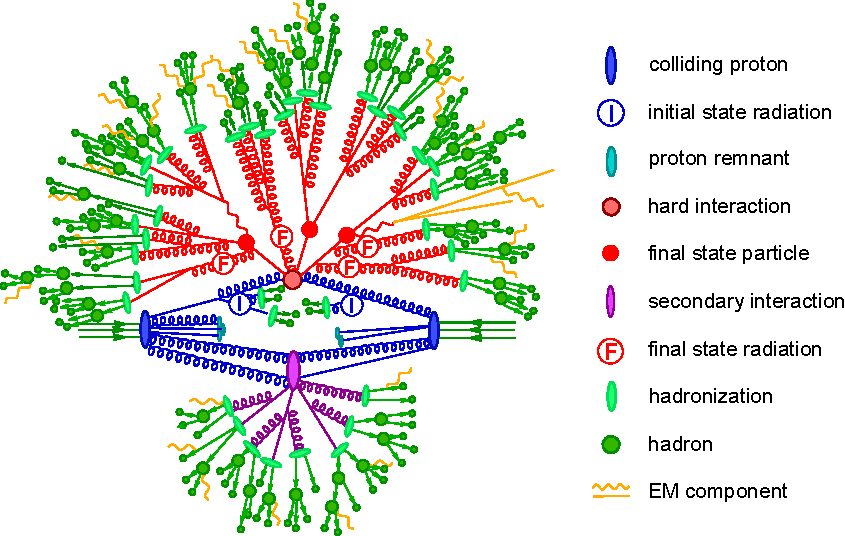
\includegraphics[scale=0.75]{figures/technique/shower.pdf}
}

A brief overview of the programs used for generation and subsequent hadronization of $t$-channel single top quark production is given in the following.

\begin{description}
\item[MadGraph5\_aMC{@}NLO] The \MGAMC program~\cite{Alwall:2014hca} is a merge of the \gls{lo} \MG generator~\cite{Alwall:2011uj} and \AMC into a common framework. It supports the generation of \gls{lo} or \gls{nlo} samples which can be matched to parton showers using the MLM~\cite{Mangano:2006rw} or MC{@}NLO~\cite{Frixione:2002ik} schemes respectively. The latter method produces a certain fraction of events with negative weights (depending on the process) which stem from a subtraction of additional emissions from the \gls{nlo} matrix element to prevent double-counting. 
Multiple samples of events with additional final state partons at matrix element level can also be merged into a combined sample. Here, the overlap with the \gls{ps} is removed through the FxFx merging scheme~\cite{Frederix:2012ps}.

\item[Powheg] The \POWHEG box (versions~1,2)~\cite{Alioli:2010xd} is a program that contains predefined implementations of various processes such as $t$-channel single top quark production~\cite{Alioli:2009je} at \gls{nlo}. It utilizes the so-called \POWHEG method~\cite{Frixione:2007vw} for matching in which the hardest radiation generated from the \gls{me} has priority over subsequent \gls{ps} emissions. This removes the overlap with the \gls{ps} without the generation of negatively weighted events.

\item[CompHEP] The \COMPHEP program (version~4.5)~\cite{Boos:2004kh} can perform calculations of cross sections from Lagrangians at \gls{lo}. In addition, generation of events is also possible such as single top quark production~\cite{Boos:2006af}. Here, an approximation is used by combining events from the $2\to2$ and $2\to3$ processes which reproduces effectively \gls{nlo} corrections.

\item[Tauola] \todo{?}

\item[Pythia] The \PYTHIA program (versions~6,8)~\cite{Sjostrand:2006za,Sjostrand:2014zea} can generate events of various processes at \gls{lo}. It is however famous for its \gls{ps} simulation which can be interfaced with other \gls{lo} and \gls{nlo} event generators to perform subsequent parton showering, hadronization, and the simulation of the underlying event. For hadronization, a phenomenological model is utilized in which one-dimensional strings\footnote{The string model is motivated by the fact that the spatial form of a dipole color field does not extend radially like an \gls{em} field but is instead squeezed to a tube-like form.} connected to partons reflect the color field leading to the creation of additional partons through string branching and finally to the formation of color-neutral singlets.

\item[Herwig++] The \HERWIG program (version~7)~\cite{Bellm:2015jjp} is an \gls{nlo} event generator which is also capable of simulating the showering of partons similar to \PYTHIA. Its hadronization algorithm utilizes a model in which color-connected quarks are spatially kept together in clusters~\cite{Webber:1983if} which is motivated by the ``preconfinement'' of color~\cite{Amati:1979fg}. If the mass of a cluster is sufficiently high it can decay into lighter clusters with a certain probability. In its final step, a cluster decays then into a pair of hadrons.
\end{description}




%##############################################
\section{Top quark reconstruction}
%##############################################

After the reconstruction and selection of analysis objects, a top quark candidate is reconstructed in the presented analyses. Assuming that the top quark decayed leptonically as $\mathrm{t}\to\mathrm{b}\mathrm{W}\to\mathrm{b}\ell\nu$ its energy and momentum is reconstructed by summing the measured 4-momenta of a selected lepton (muon or electron), b-tagged jet, and neutrino candidate. The neutrino candidate itself is reconstructed from the missing transverse energy and the lepton momentum by requiring a W~boson mass constraint of $m_\mathrm{W}=80.4~\GeV$~\cite{Olive:2016xmw} on their invariant mass as

\begin{align}
m_\mathrm{W}^2=\colvec{2}{E_\mathrm{W}}{\vec{p}_\mathrm{W}}^{2}&\overset{!}{=}\left[\colvec{2}{E_{\ell}}{\vec{p}_{\ell}}+\colvec{2}{E_{\nu}}{\vec{p}_{\nu}}\right]^{2}\nonumber\\
&=\underbrace{m_{\ell}^2+m_{\nu}^2}_{\approx 0}+\,2\cdot E_{\ell}\,E_{\nu}-\,2\cdot\colvec{3}{p_{\ell,x}}{p_{\ell,y}}{p_{\ell,z}}\cdot\colvec{3}{p_{\nu,\mathrm{T}}\cdot\cos\phi_{\nu}}{p_{\nu,\mathrm{T}}\cdot\sin\phi_{\nu}}{p_{\nu,z}}. \label{eq:technique-neutrino-pz-eq}
\end{align}

When taking $p_{\nu,\mathrm{T}}$ and $\phi_{\nu}$ from the missing transverse momentum vector $\pvmiss$, this allows to solve for the unknown $p_{\nu,z}$-component of the neutrino candidate momentum. After rearranging, one obtains from Eq.~\ref{eq:technique-neutrino-pz-eq} the quadratic equation

\begin{equation}
0=p_{\nu,z}^2-\frac{2\,\xi\,p_{\ell,z}}{E_{\ell}^{2}-p_{\ell,z}^2}\cdot p_{\nu,z}-\frac{\xi^{2}-E_{\ell}^{2}\,p_{\nu,\mathrm{T}}^2}{E_{\ell}^{2}-p_{\ell,z}^2},\end{equation}

with

\begin{equation}
\xi=\frac{m_\mathrm{W}^2}{2}+p_{\nu,\mathrm{T}}\,p_{\ell,\mathrm{T}}\cdot\cos\big(\phi_\ell-\phi_\nu\big)
\end{equation}

which possesses the solutions

\begin{align}
p_{\nu,z}^{1,2}=\frac{1}{E_{\ell}^{2}-p_{\ell,z}^{2}}\left[\xi\cdot p_{\ell,z}\pm E_{\ell} \sqrt{\xi^2-p_{\nu,\mathrm{T}}^2\big(E_{\ell}^2-p_{\ell,z}^2\big)}~\right]. \label{eq:technique-neutrino-pz}
\end{align}

A detailed derivation and discussion of this result can be found in Ref.~\cite{Chwalek:1416031}. In simulated $t$-channel single-top-quark events this procedure leads to two real solutions for the neutrino $p_{\nu,z}$-component in about 65\% of all events that passed the selection. The difference of the two real solutions with respect to the true neutrino $p_{z}$ at parton level is displayed in Fig.~\ref{fig:technique-neutrino-reco}. 

\myfigure{\label{fig:technique-neutrino-reco}Differences of the reconstructed neutrino $p_{z}$ with respect to the neutrino $p_{z}$ at parton level in cases of real and complex solutions. The distributions have been generated using \POWHEG interfaced with \TAUOLA and \PYTHIA8.}{
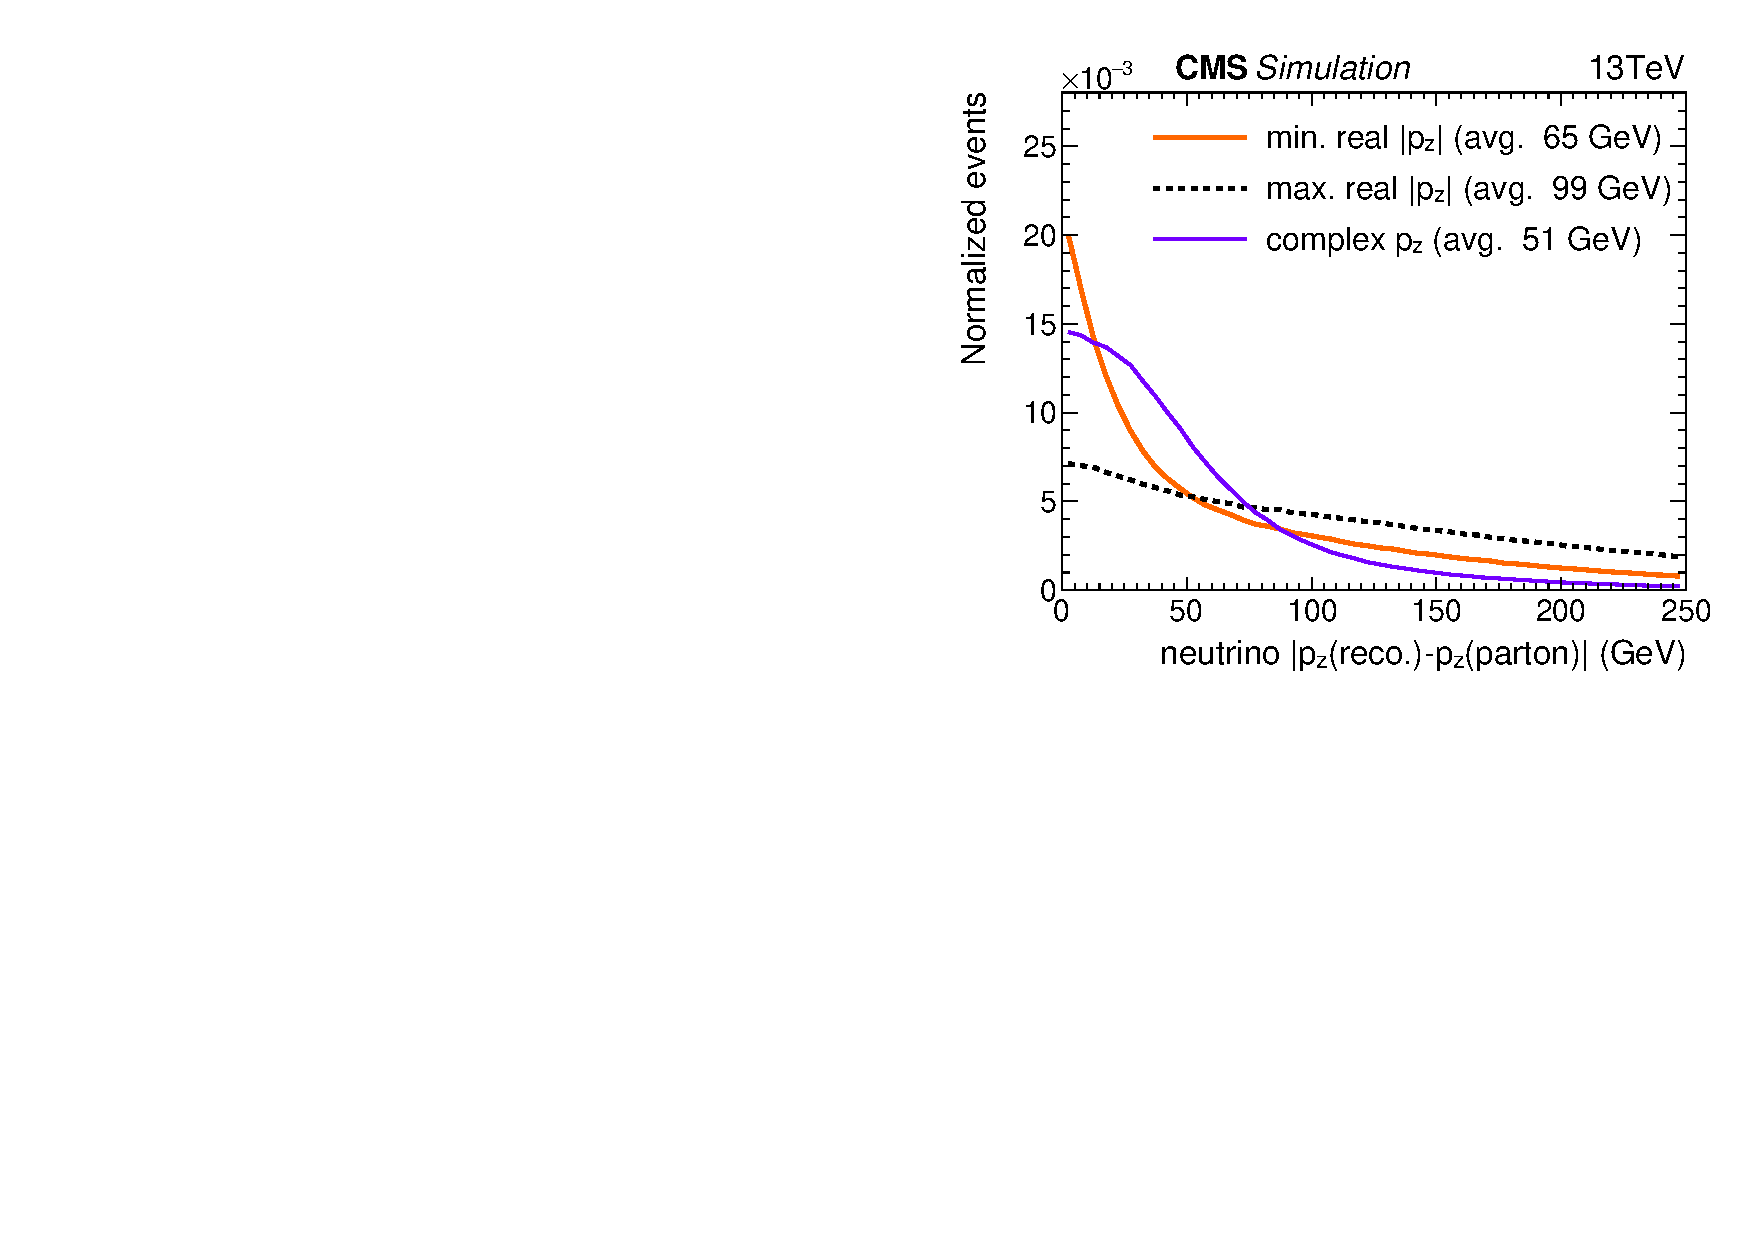
\includegraphics[width=0.52\textwidth]{figures/technique/neutrino_match_dpz.pdf}
}

The plot demonstrates that choosing the solution which has the smallest absolute $|p_{\nu,z}|$ yields on average a neutrino $p_{z}$ which is closest to the true neutrino $p_{z}$. If the discriminant in Eq.~\ref{eq:technique-neutrino-pz} becomes negative the solutions are complex. This happens in about 35\% of events and occurs mostly due to the finite \met resolution whereas the negligence of the W~boson mass width and resolution of the lepton momentum are minor effects. The imaginary part of the solutions is removed by requiring that the discriminant vanishes

\begin{equation}
0\overset{!}{=}\xi^2-p_{\nu,\mathrm{T}}^2\big(E_{\ell}^2-p_{\ell,z}^2\big)~
\Rightarrow~ p_{\nu,z}=\frac{\xi\cdot p_{\ell,z}}{E_{\ell}^{2}-p_{\ell,z}^{2}}
\end{equation}

which is equal to setting the transverse W~boson mass $\mtw$ to the W~boson mass itself

\begin{align}
m_\mathrm{W}^2\overset{!}{=}\mtw^2&=(p_{\ell,\mathrm{T}}+p_{\nu,\mathrm{T}})^2-(p_{\ell,x}+p_{\nu,x})^{2}-(p_{\ell,y}+p_{\nu,y})^{2}\\
&=2\,p_{\ell,\mathrm{T}}^2\,p_{\nu,\mathrm{T}}^2\cdot\Big[1-\cos\big(\phi_\ell-\phi_\nu\big)\Big].
\end{align}

Then, the $p_{\nu,x}$ and $p_{\nu,x}$ components are varied and the transverse momentum which minimizes the distance $|\vec{p}_{\nu,\mathrm{T}}-\pvmiss|$ with respect to the measured missing momentum vector is taken as the result. 

After finding a solution for the unknown neutrino $p_{z}$ component, a top quark candidate can be constructed from the 4-momenta of the lepton, b-tagged jet, and neutrino candidate. Shape comparisons of the top quark mass and pseudorapidity for the two neutrino solution cases are presented in Fig~\ref{fig:technique-top-reco}. In the case that only a complex solution has been found an improved reconstructed top quark mass resolution is achieved. Similarly, the pseudorapidity of the top quark candidate demonstrates an improved reproduction of the corresponding observable at parton level as well.

\myfigure{\label{fig:technique-top-reco} Shape differences in the reconstructed top quark (a)~mass and (b)~pseudorapidity for cases with real neutrino $p_{z}$ solutions where the one with the smallest $|p_{z}|$ is picked or only a complex solution. The distributions have been generated using \POWHEG interfaced with \TAUOLA and \PYTHIA8.}{
\subfloat[]{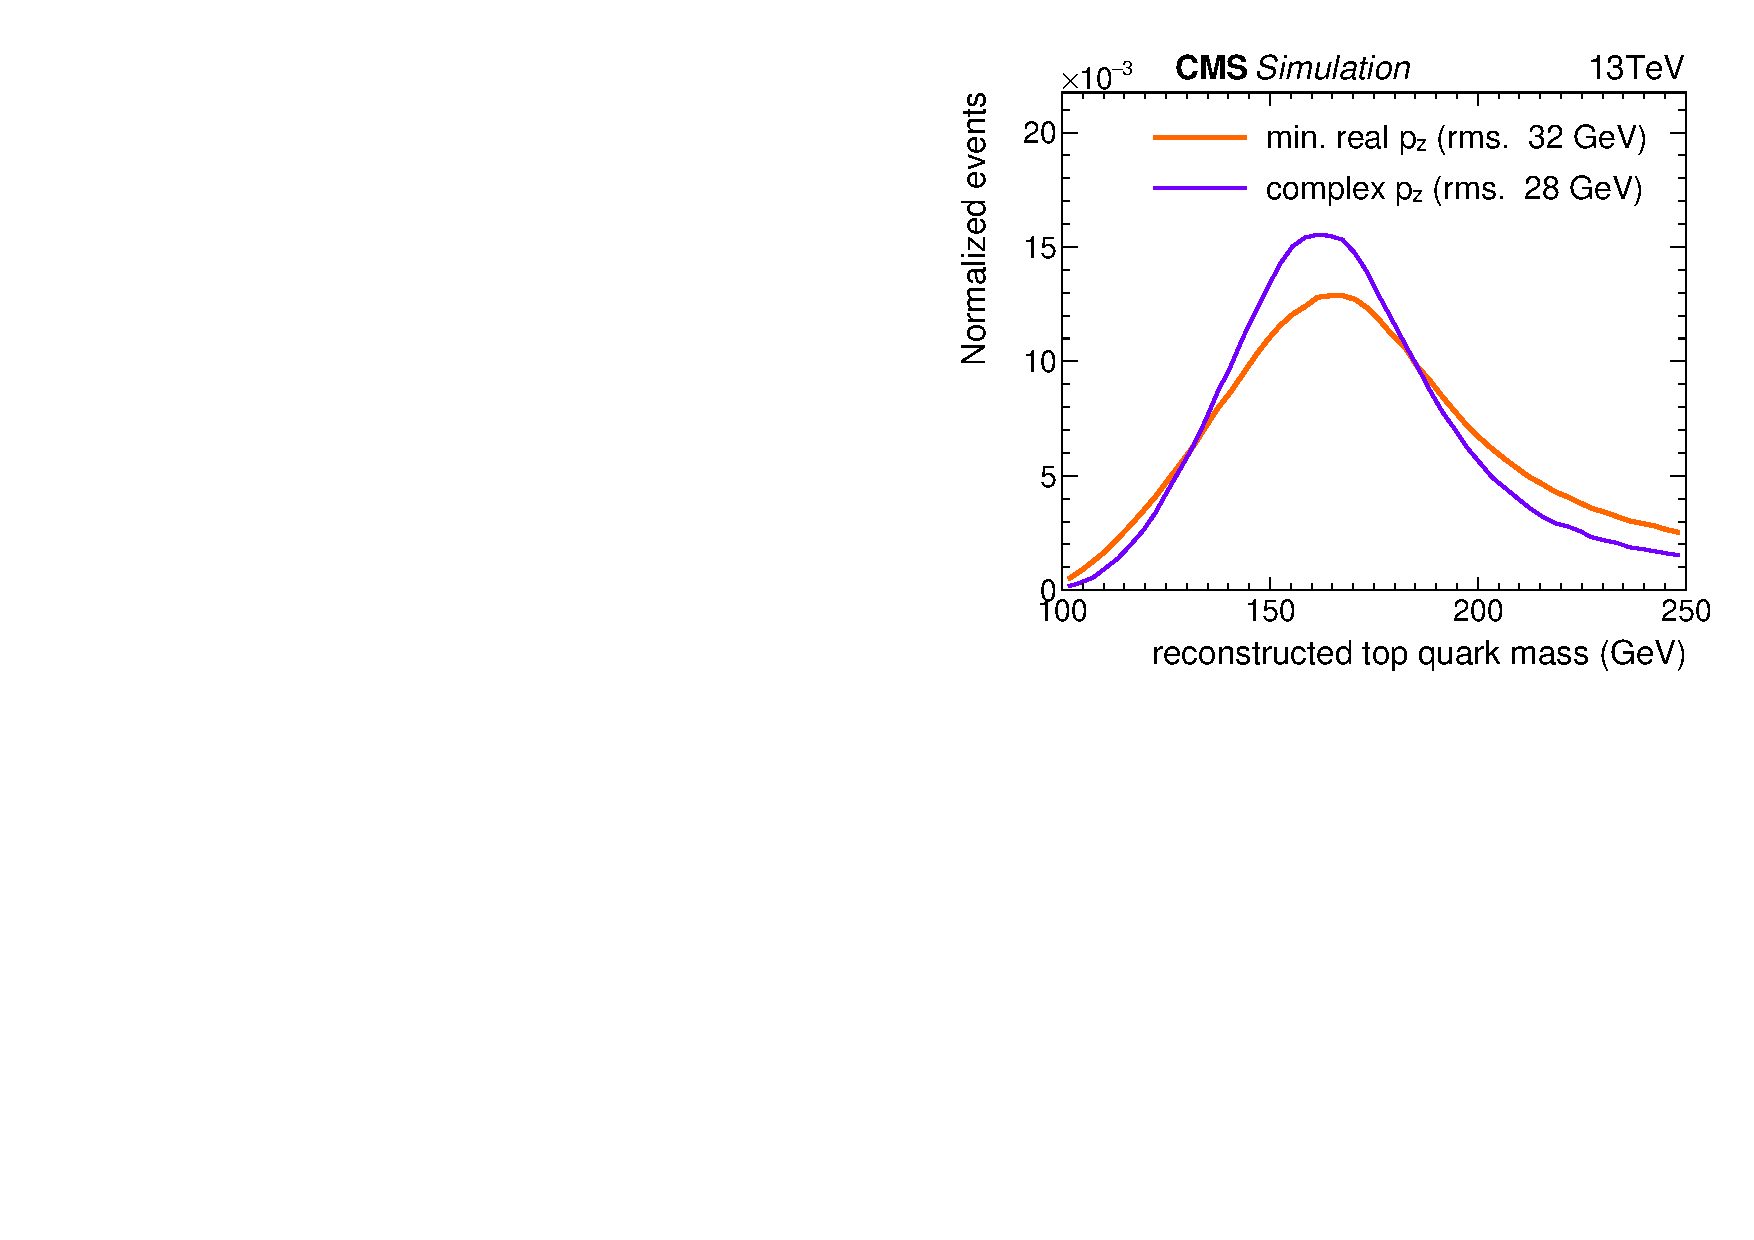
\includegraphics[width=0.48\textwidth]{figures/technique/top_match_mass.pdf}}\hspace{0.03\textwidth}
\subfloat[]{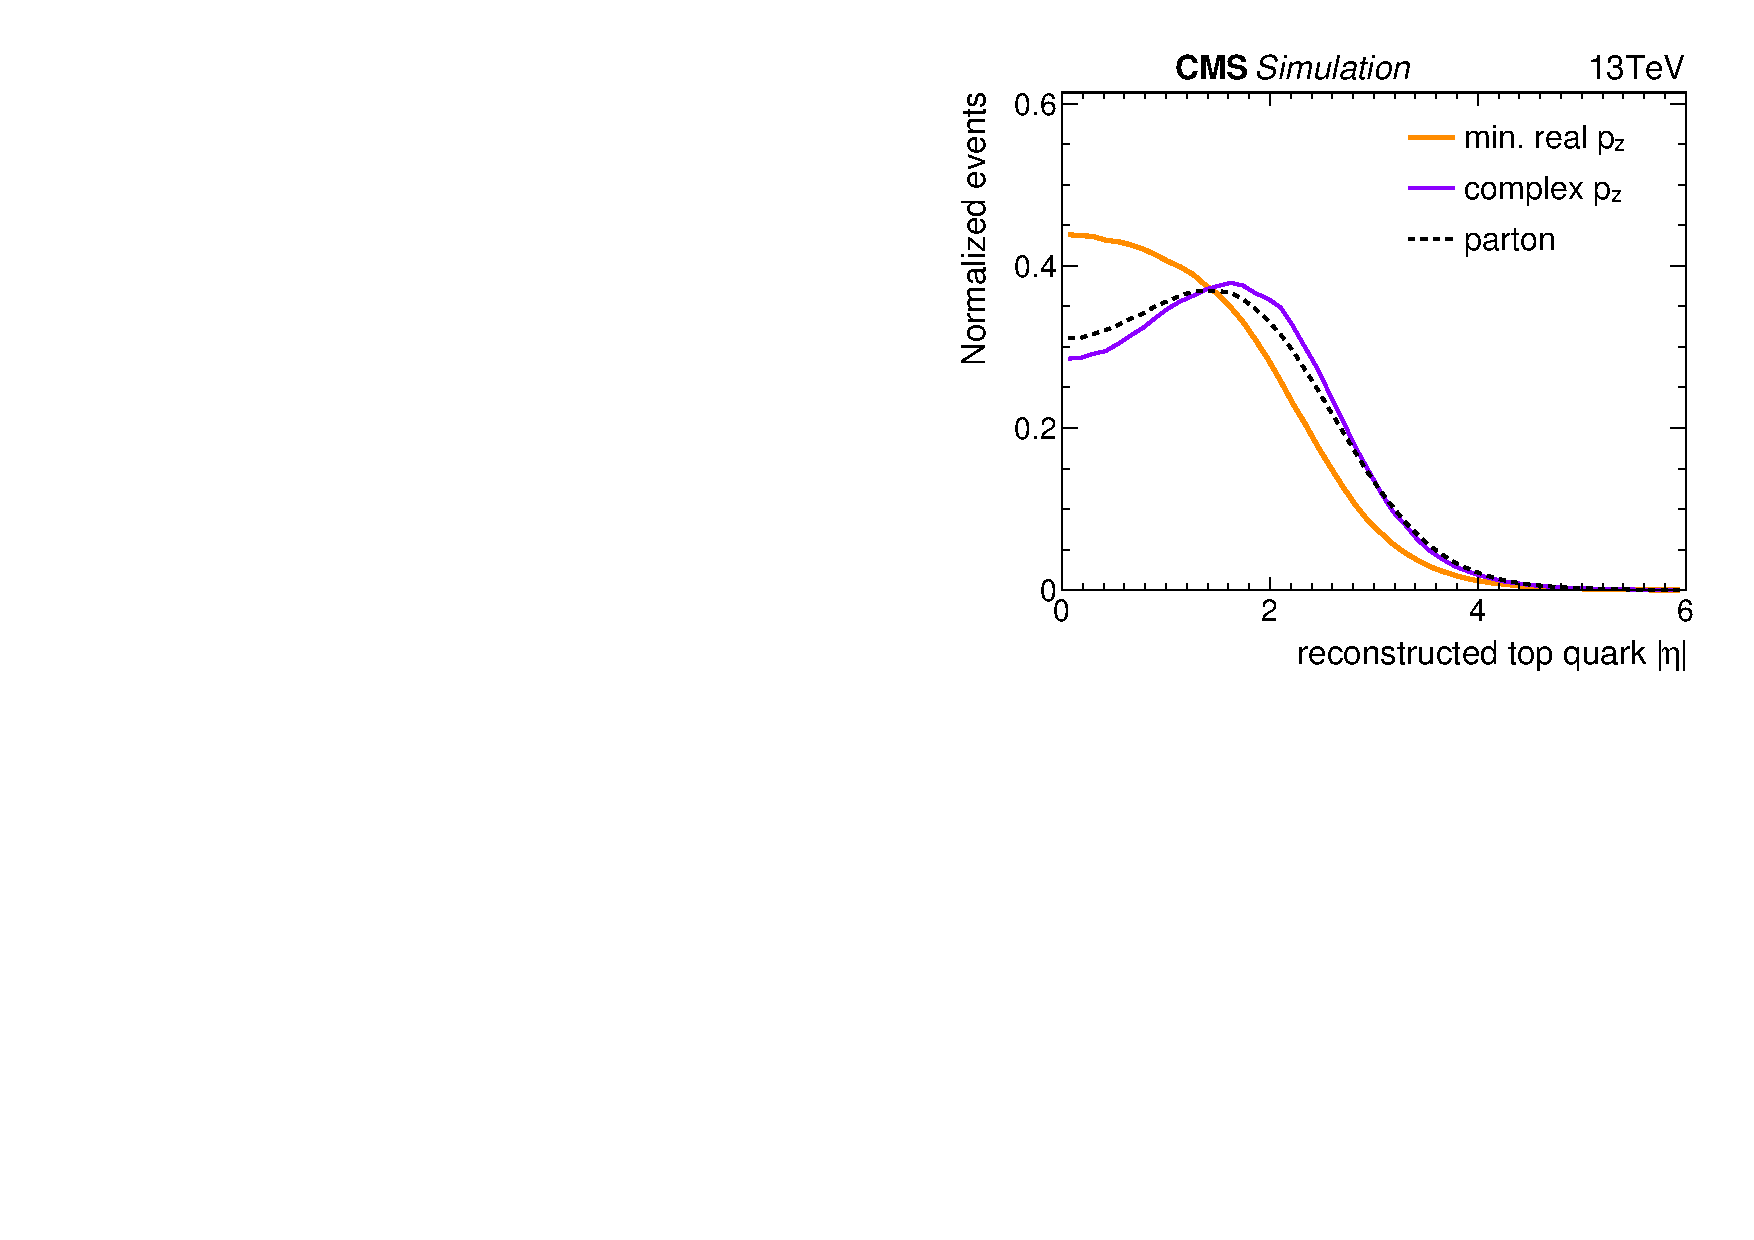
\includegraphics[width=0.48\textwidth]{figures/technique/top_match_eta.pdf}}
}

\todo{top quark matching performance
(top pT/eta as function of b-tag in acceptance after selection, b-quark within dR, top within dR)}

%##############################################
\section{Boosted Decision Trees}
%##############################################

The $t$-channel single-top-quark signal region, defined by one isolated lepton, 2~jets (where one is b-tagged), and significant \met, is found to be still largely contaminated by events from background processes after the event selection. The \glshere{sb} yield ratios are about 13\% and 14\% in analyses at 8~and 13~TeV, respectively~\cite{Khachatryan:2014iya,Sirunyan:2016cdg}\todo{update TOP-16-003 when accepted by PRL}. The majority of background events stems from \wjets, \ttbar, and multijet production whereas contributions from single top quark tW and $s$-channel, Drell-Yan, and diboson production are minor. The small \gls{sb} ratio motivates the usages \glshere{mva} techniques. In this thesis, \glsplhere{bdt} are employed for event classification as implemented in the \gls[]{tmva} framework~\cite{Hocker:2007ht}. They are based on a set of decision trees where each yields a binary output depending on whether an event is signal- or background-like. Their training and how the single decision tree outputs are combined into a one-dimensional discriminant are detailed in the following.

An exemplary decision tree is presented in Fig.~\ref{fig:technique-decisiontree} where sequential selections on observables $x_{i}$ are applied such that the leaf nodes contain either a majority of signal or background events. Such a tree is build from samples of simulated events for which the desired classification is a priori known~(``superivsed learning'').

\myfigure{\label{fig:technique-decisiontree} A sketch of a decision tree.}{
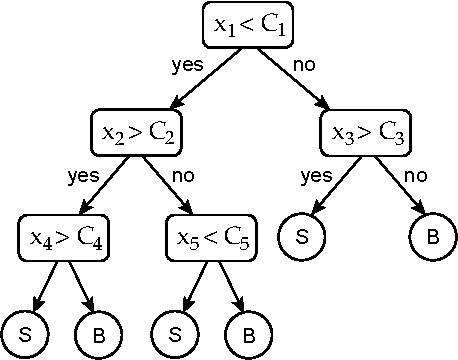
\includegraphics[scale=0.75]{figures/technique/decision_tree.pdf}
}

By maximizing the separation between the signal and background distributions per node the optimal observable $x_{i}$ and working point $C_{i}$  are found. In the analyses, the separation is calculated as the cross entropy 

\begin{align}
H&=-p\cdot\ln(p)-(1-p)\cdot\ln(1-p)\\ p_{i}&=\frac{\int_{C_{i}}^{\infty} N_\mathrm{sig.}(x_{i})\,\mathrm{d}x_{i}}{\int_{C_{i}}^{\infty} N_\mathrm{sig.}(x_{i})+N_\mathrm{bkg.}(x_{i})\,\mathrm{d}x_{i}}\\
\Rightarrow &~\{x_{i},\,C_{i}\}=\max\Big(H\,\big|~x_{i},\,C_{i}\Big)
\end{align}

where $p$ denotes the achieved purity of a selection $x_{i}>C_{i}$. Other common measures of separation are the misclassification error or the so-called ``Gini'' index~\cite{Gini}. The separation measures are constructed to be symmetric when swapping the signal and background classes since obtaining a background leaf with high purity is of equal importance. A node is not split if it contains less than a predefined minimum number of events to ensure that the decisions per node and the binary outputs per leaf are statistically significant. This also mitigates a potential ``overtraining'' of a decision tree which occurs when statistical fluctuations are learned instead of the underlying physical distributions due to the finite statistics of the training sample. Additional caution is required when using a sample which contains a portion of negatively weighted events~(e.g. generated with \MGAMC). In such a case, a tree may be trained incorrectly if a large fraction of negatively weighted events are selected in one of the nodes since the distributions of observables can contain regions with unphysical yields. To tweak the cancellation of negatively weighted events the minimum number of events can be increased further beyond the statistical motivated threshold one would choose when training only on a sample of purely positively weighted events. In addition, the working point values per observable which are analyzed to find the optimal node splitting can be preset which prevents that a decision becomes sensitive to single events close to the selection border.

Single decision trees can still be perceptible to statistical fluctuation leading to misclassification errors when given a statistically-independent test sample. This is mitigated by training multiply decision trees with binary outputs $h_{i}\in\{-1,1\}$ that are then combined into a pseudo-continuous discriminant using a majority vote as

\begin{equation}
M(\vec{x})=\sum_{i}^{N_\mathrm{trees}}~w_{i}\cdot h_{i}\,(\vec{x};\,\vec{C}_{i}).\label{eq:technique-majority-vote}
\end{equation}

Here, each decision tree output is multiplied by a so-called boosting weight $w_{i}$. This way of combining multiple decision trees has another advantage. It has been shown that the majority vote can yield a classifier with high accuracy by applying a ``boosting'' procedure. Such a ``strong learner'' can already be obtained if the individual decision trees are just ``weak learners'' which means that they have only a low classification accuracy~\cite{Schapire1990,FREUND1995256}. The decision trees can therefore be kept very shallow, e.g. only two or three layers of selections, which also improves their robustness against overtraining. A boosting procedure accounts then for the individual accuracy per tree by adjusting its weight accordingly in the majority vote which results into a strong learner.

The two boosting procedures employed in this thesis are the adaptive boosting, \ADABOOST~\cite{FREUND1997119}, and \GRADIENTBOOST~\cite{Friedman00greedyfunction} algorithms. In the \ADABOOST algorithm, decision trees are trained iteratively. At each step, a single decision tree is trained and the misclassified events are identified. Their weight is then increased in the training of subsequent trees by the boosting weight

\begin{equation}
\alpha_{n+1}=\left(\frac{1-\epsilon_{n}}{\epsilon_{n}}\right)^\beta
\end{equation}

where $\epsilon_{i}$ denotes the misclassification rate of the current tree $n$ and $\beta$ is a configurable learning rate. The corresponding weight in Eq.~\ref{eq:technique-majority-vote} is then given by $w_{i}=\ln\alpha_{i}$. Typically, a slow learning rate of $\beta\leq0.5$ is chosen to allow for more boosting steps. It can be shown that the \ADABOOST algorithm is equivalent to the minimization of the exponential loss function $L(M,y)=\exp(-M(\vec{x})\,y)$ where $y$ denotes the true classification of events~\cite{Hocker:2007ht}. If the loss function is instead changed to 

\begin{equation}
L(M,y)=\ln\left(1+e^{-2\,M(\vec{x})\,y}\right)
\end{equation}

the \GRADIENTBOOST algorithm is obtained. Its loss function is more robust in the presence of outliers and noise events for which the \ADABOOST algorithm may degrade. The algorithm commences by iteratively minimizing the loss function with respect to the weights and decision tree parameters in $M$ using the method of gradient decent. During the minimization steps, the output of the majority vote will gradually tend towards $y$ because misclassified events result in large gradients of the loss function. Similar to the \ADABOOST algorithm, an increased performance is obtained when decreasing the learning rate controlling the boosting weights which is called ``shrinkage'' here. In this thesis, both boosting algorithms have been tested to validate their performances with respect to each other. Only negligible differences in their discrimination power have been found after optimizing their training parameters.

The discrimination power of a trained \gls{bdt} is assessed by analyzing the \glshere{roc} curve. Exemplary \gls{roc} curves are presented in Fig.~\ref{fig:technique-bdt-rocs}. The \gls[]{auc} values denote the area under the \gls{roc} curve with respect to random guessing. Here, the \gls{roc} curves of a \gls{bdt} trained to discriminate $t$-channel single-top-quark events against \wjets and \ttbar background events is compared to the pseudorapidity of the untagged light jet and to the reconstructed top quark mass difference. An \gls{auc} of about $32\%$ is achieved with the trained \gls{bdt} which outperforms the other two typical event observables for separating $t$-channel events from background processes. The exact setup of the \gls{bdt} shown here will be discussed in Sec.~\ref{sec:diff13-bdt} together with the corresponding analysis.

\myfigure{\label{fig:technique-bdt-rocs}Comparison of \gls{roc} curves for separating $t$-channel single-top-quark events from background events (\wjets, \ttbar) using: random guessing; a trained \gls{bdt} discriminant; the pseudorapidity of the untagged light jet ($\jprime$); the difference of the reconstructed top quark mass with respect to the nominal mass, $\Delta m_\mathrm{top}=m_\mathrm{top}-172.5~\GeV$.}{
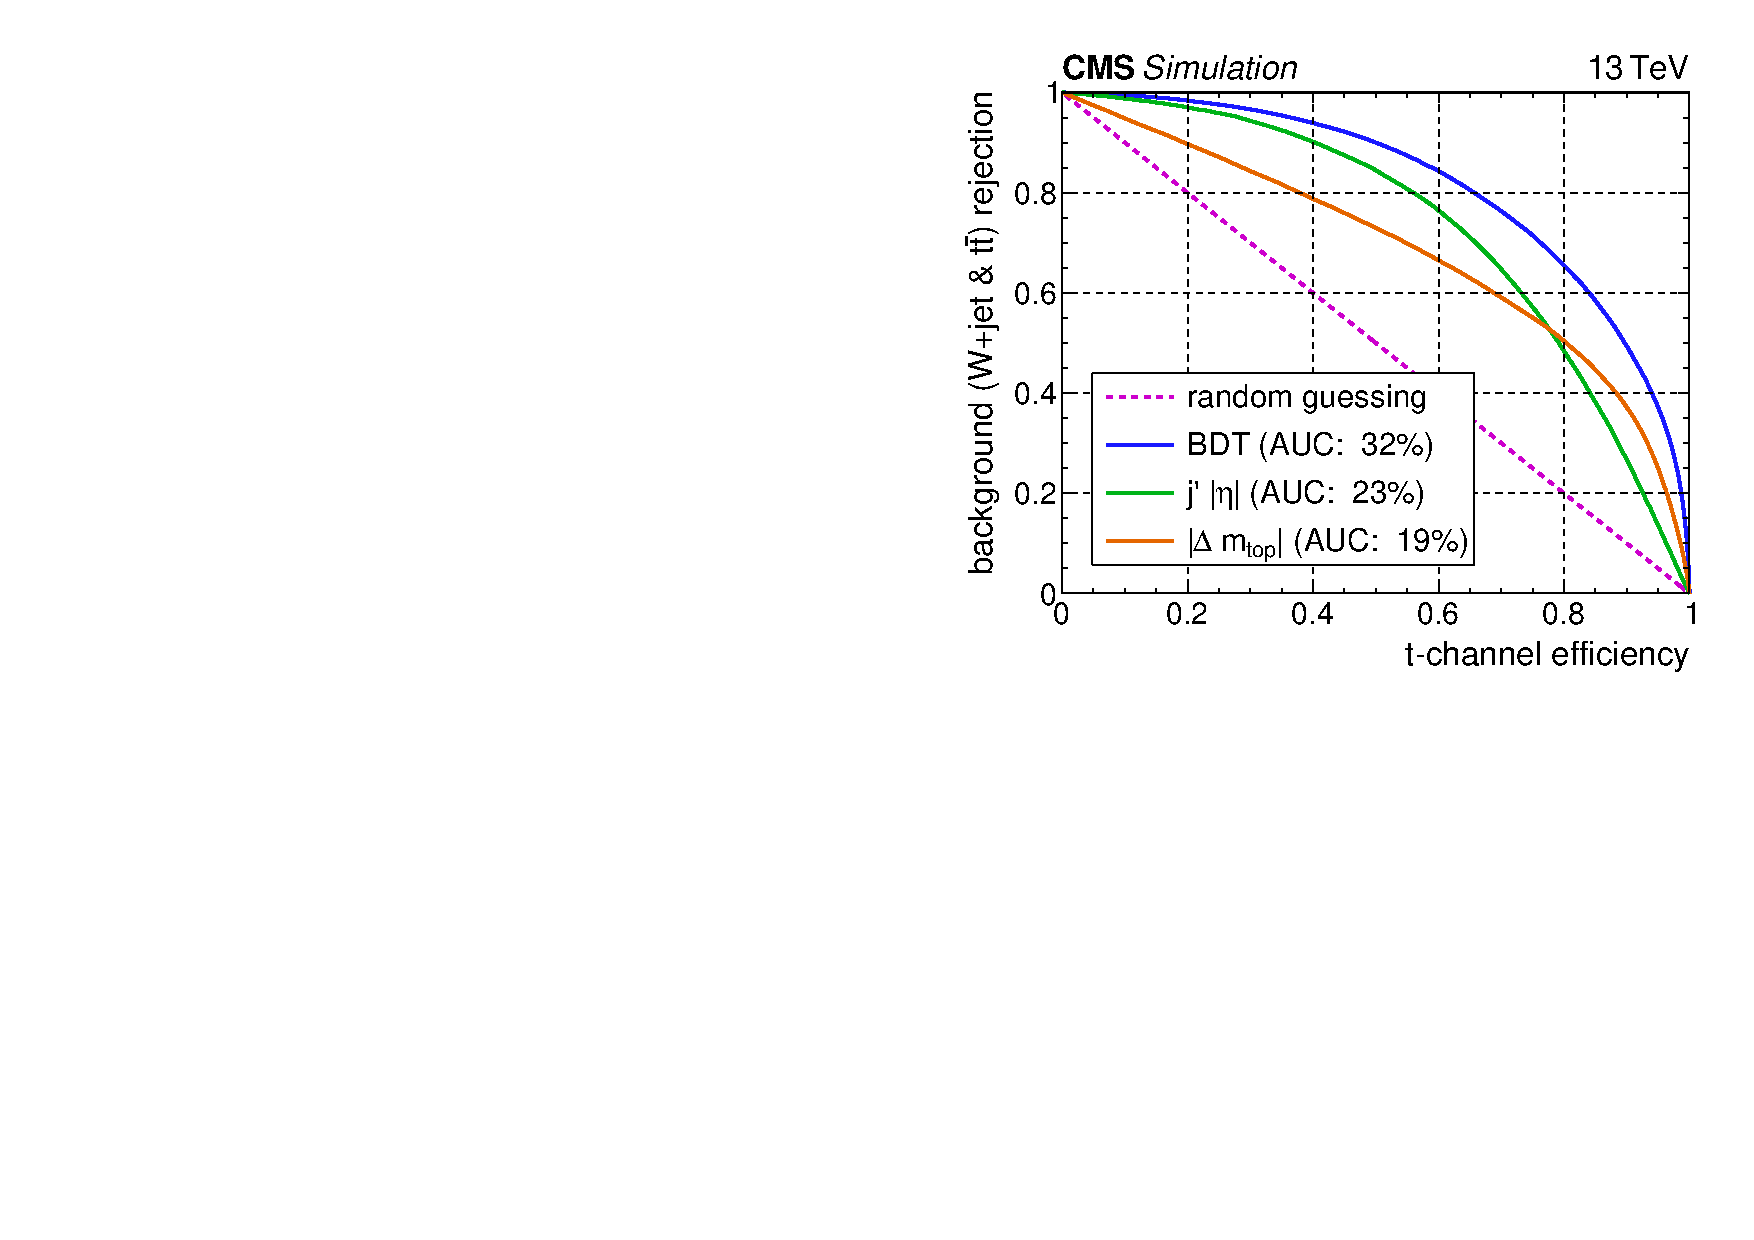
\includegraphics[width=0.5\textwidth]{figures/technique/rocs.pdf}
}


%##############################################
\section{Template-based fitting}
%##############################################

In the analyses, the amount of signal and background events is estimated from data using template-based \glshere{ml} fits. For an observable to be fitted, histograms of simulated events act as templates which reflect the expected distributions of events per process. The likelihood that the observed distribution in data is a realization of the expectation from simulation can then be expressed as

\begin{equation}
\mathsf{L}_\mathrm{Poi.}=\prod_{i}^\mathrm{bins}~\frac{p_{i}^{\,d_{i}}\cdot e^{-p_{i}}}{d_{i}!},\qquad p_{i}=\beta^{\mathrm{(sig.)}}\cdot t^{\mathrm{(sig.)}}_{i}+\sum_{j}^\mathrm{bkgs.}~\beta^{(j)}\cdot t^{(j)}_{i}. \label{eq:technique-likelihood}
\end{equation}

The amount of observed data events $d_{i}$ per bin $i$ is modeled to follow a Poisson distribution with an expected event yield $p_{i}$. The expected yields are obtained by summing the respective contributions of the signal and background templates $t^\scriptn{(X)}_{i}$ per process $X$. The normalization per process is controlled through scale factors $\beta^\scriptn{\mathrm{(X)}}$. These are then estimated through the fit from data by maximizing the likelihood. The signal scale factor is also referred to as signal ``strength'' whereas the background scale factors are sometimes called nuisance parameters because their estimation is of less importance. Technically, the \THETA framework~\cite{theta} is employed for template-based fitting where for convenience and numerical stability reasons the negative logarithm of the likelihood

\begin{equation}
-\ln\Big(\mathsf{L}_\mathrm{Poi.}\big(\vec{\beta}\big)\Big)=-\sum_{i}^\mathrm{bins}~\Big[\,d_{i}\ln p_{i}\big(\vec{\beta}\big)-p_{i}\big(\vec{\beta}\big)\Big]+\mathrm{const.}
\end{equation}

is minimized which is however equivalent to maximizing Eq.~\ref{eq:technique-likelihood} with respect to the scale factors. Since the templates are normalized to their corresponding \gls{sm} cross sections times the integrated luminosity, an estimated scale factor can be directly translated into a corresponding cross section as

\begin{align}
\hat{\sigma}_\mathrm{sig.}&=\frac{\hat{N}_\mathrm{sig.}}{A\cdot\epsilon\cdot{\textstyle{\int}L}}~,\quad
\hat{N}_\mathrm{sig.}=\hat{\beta}_\mathrm{sig.}\cdot N_\mathrm{exp.}=\hat{\beta}_\mathrm{sig.}\cdot\underbrace{\sigma_\mathrm{\gls{sm}}\cdot\textstyle{\int}L}_\mathrm{normalization}\cdot \overbrace{A \cdot \epsilon}^\mathrm{selection}\nonumber\\
&=\hat{\beta}_\mathrm{sig.}\cdot\sigma_\mathrm{\gls{sm}}
\end{align}

where $A$ denotes the acceptance and $\epsilon$ the efficiency of the event selection which are intrinsically estimated through the simulated samples. For the background scale factors additional constraints are applied by adding log-normal priors to the likelihood as

\begin{equation}
-\ln\Big(\mathsf{L}_\mathrm{bkgs.}\Big)=\sum_{j}^\mathrm{bkgs.}~\frac{1}{2}\cdot\left(\frac{\ln\,\beta^{(j)}}{\delta^{(j)}}\right)^{2}.
\end{equation}

These additional constraints with uncertainties $\delta$ reflect a priori believes of the background contributions in the signal phase space where the fit is carried out. They are motivated by the fact that the selected analysis phase space is usually only optimized to measure the signal process accurately but not the background contributions. Here, log-normal distributions are explicitly preferred to model the constraints over Gaussian distributions because in the case of large uncertainties log-normal distributions will not be biased when requiring that the scale factors are always positive. For Gaussian distributions with large widths, such a truncation shifts the mean of the distribution which then biases the fit result.

In the fit, an extra uncertainty is considered to account for the limited accuracy of the predicted event yields per bin due to the finite statistics of the simulated event samples. A method proposed by R. Barlow and C. Beeston~(\gls[]{bb})~\cite{Barlow:1993dm} is to model this uncertainty by adding additional nuisance parameters $\nu_{ij}$ for each bin $i$ and process $j$ which modifies the predicted yields as $p_{i}^\prime=\sum_{j}\nu_{ij}\cdot p_{ij}$. These so-called \gls{bb} parameters are constrained in the likelihood to reflect the uncertainties of the sample statistics. This approach however increases the complexity of the fit since many more parameters have to be estimated in addition to the signal and background scale factors. The number of free parameters is reduced in the Barlow-Beeston lite method~\cite{Conway:2011in} where the uncertainties per bins are grouped and describe by only a single nuisance parameter. A further, technical simplification can be achieved when using numerical minimization algorithms for fitting. Here, it is computationally advantageous to only maximize the likelihood with respect to the scale factors while adjusting the \gls{bb} parameters adaptively to cover the remaining difference between prediction and data per bin. This approach is also implemented in the employed \THETA framework.



%##############################################
\section{Parton and particle level observables}
%##############################################

Cross sections can be measured not only inclusively but also differentially in intervals of an observable. Differential cross sections offer the means to perform in-deep comparisons of data with theoretical predictions. The result of such measurements allows to assess the modeling and validity of event generators and analytical calculations. Furthermore, as detailed in Ch.~\ref{ch:top}, some differential cross sections can be sensitive to the coupling structure of a process and can thus be interpreted in potential \gls{bsm} scenarios as well.

A proper comparison of differential cross sections can only be achieved if the corresponding observable is well-defined and identical across generators and analytical calculations. There are two ``levels'' at which physics objects of a process and related observables are typically defined. These are presented in Fig~\ref{fig:technique-parton-particle}. The parton level corresponds to the intermediate and final state particles within a Feynman diagram. In event generators, these particles are produced as the hard interaction before the event is handed to a parton shower program where result of the hadronization and various other effects~(see Fig.~\ref{fig:technique-mcevent}) are simulated. The partonic top quark is defined to be on-shell while accounting for \gls{qcd}/\gls{qed} radiations and the intrinsic $k_\mathrm{T}$ of initial state partons which may boost the event. Prompt leptons which originate from the W~boson decay are defined in the same manner. About 15\% of the final state electrons or muons originate from a leptonically decaying tau lepton, these leptons are included into the definition as well. The fraction depends on the \pt threshold of the muon or electron as depicted in Fig.~??. When selection electron or muons with a $\pt$ of at least $20~\GeV$ this the fraction of leptonically decaying tau leptons entering the selected phase space reduces to 6\%.


The spectator quark may radiate a gluon as shown exemplary. At \gls{nlo}, this can lead to an ambiguity if it is accounted

ambigous at NLO, 4/5FS because of 2nd b-quark

\textit{''The unfortunate truth is that most of the event record is intended
for generator debugging rather than physics interpretation''}~\cite{Buckley:2010ar}.

\myfigure{\label{fig:technique-parton-particle}A sketch of parton and particle level objects in $t$-channel single-top-quark production.}{
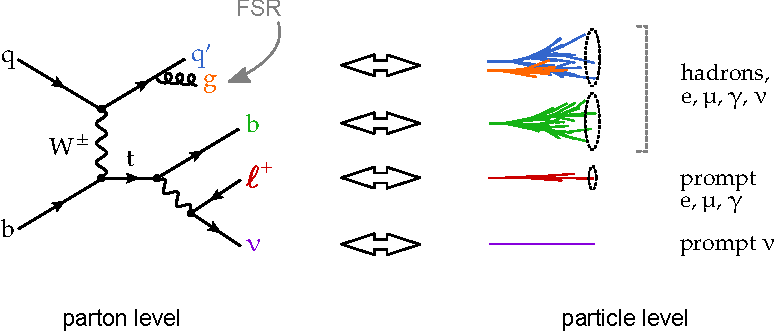
\includegraphics[scale=0.75]{figures/technique/fiducial.pdf}
}

\myfigure{\label{fig:technique-parton-muon} Distributions of the muon transverse momentum, pseudorapidity for $t$-channel single top quark production at $13~\TeV$. The distributions have been generated using \POWHEG interfaced with \TAUOLA and \PYTHIA8.}{
\subfloat[]{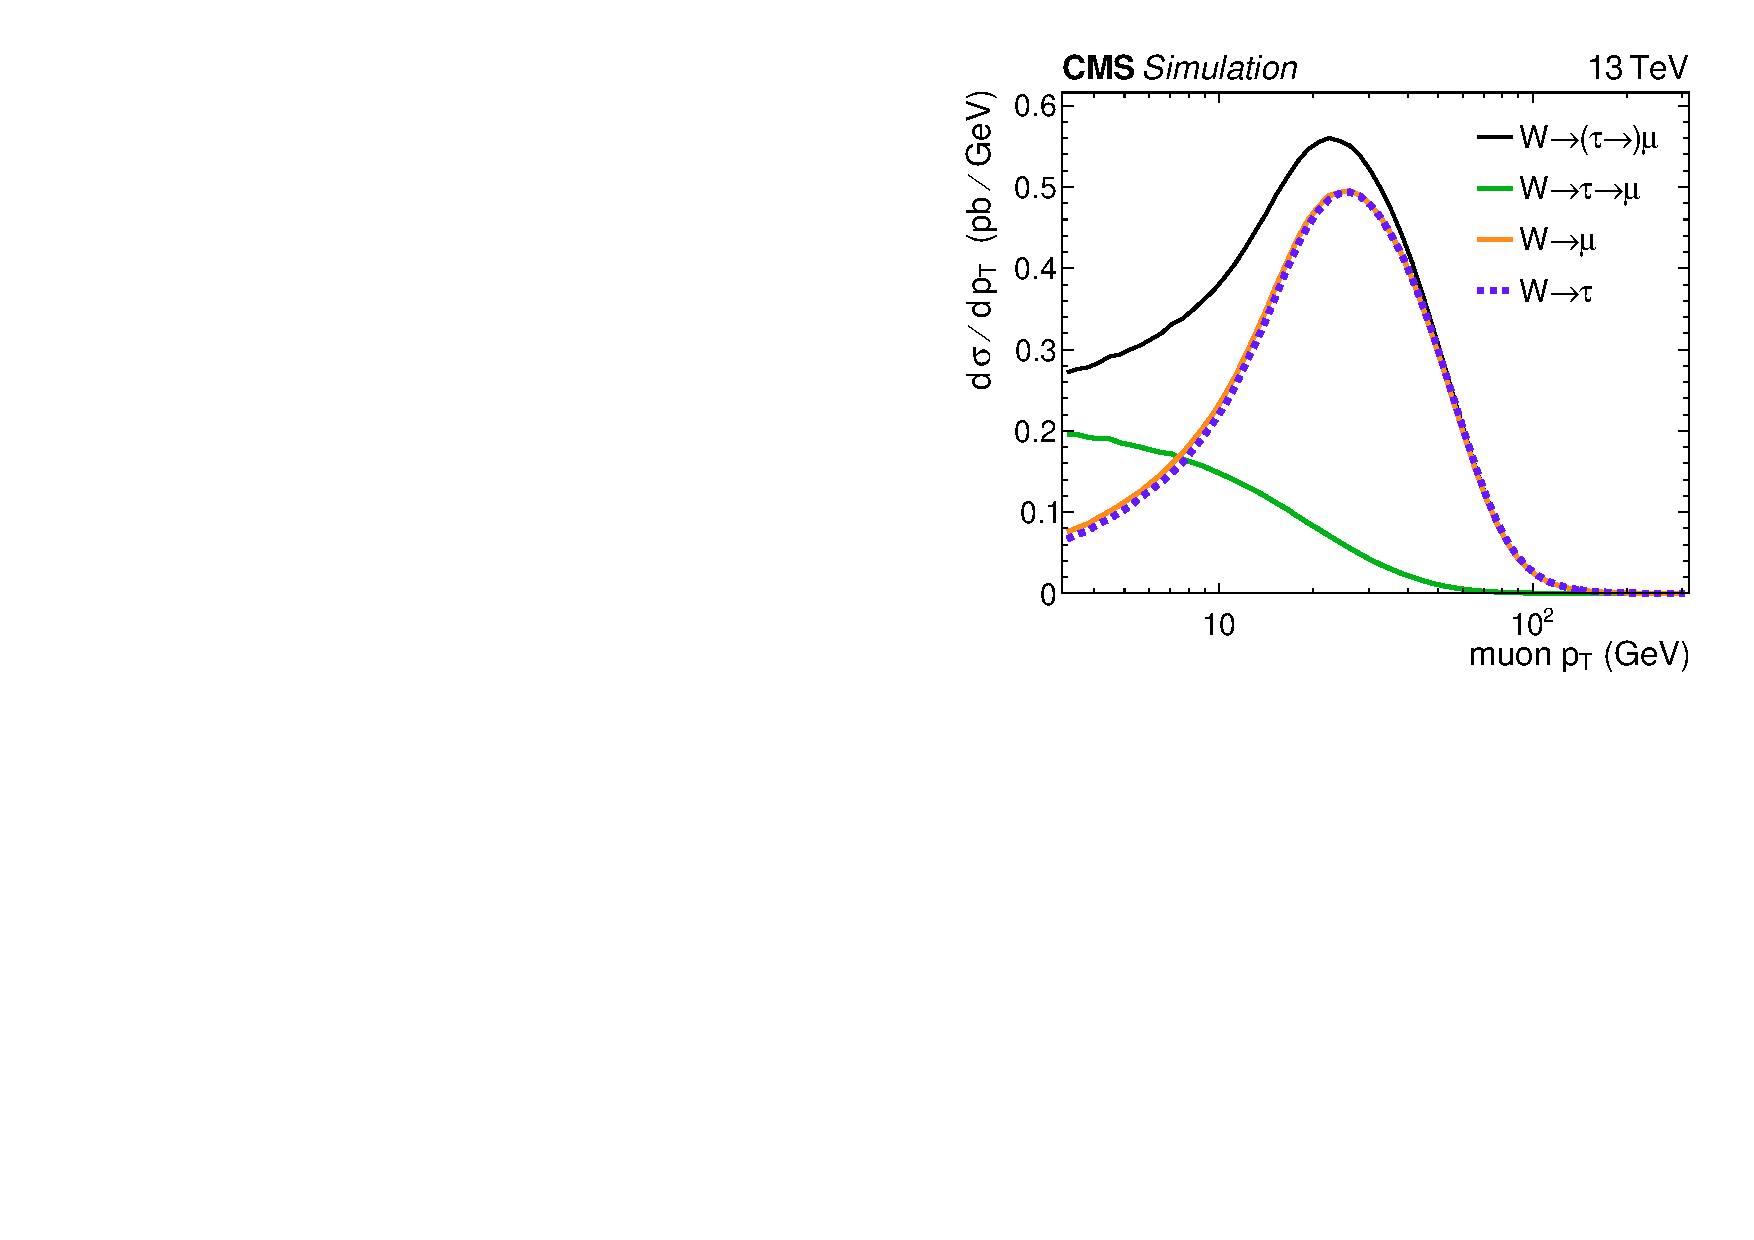
\includegraphics[width=0.48\textwidth]{figures/technique/lepton_pt.pdf}}\hspace{0.03\textwidth}
\subfloat[]{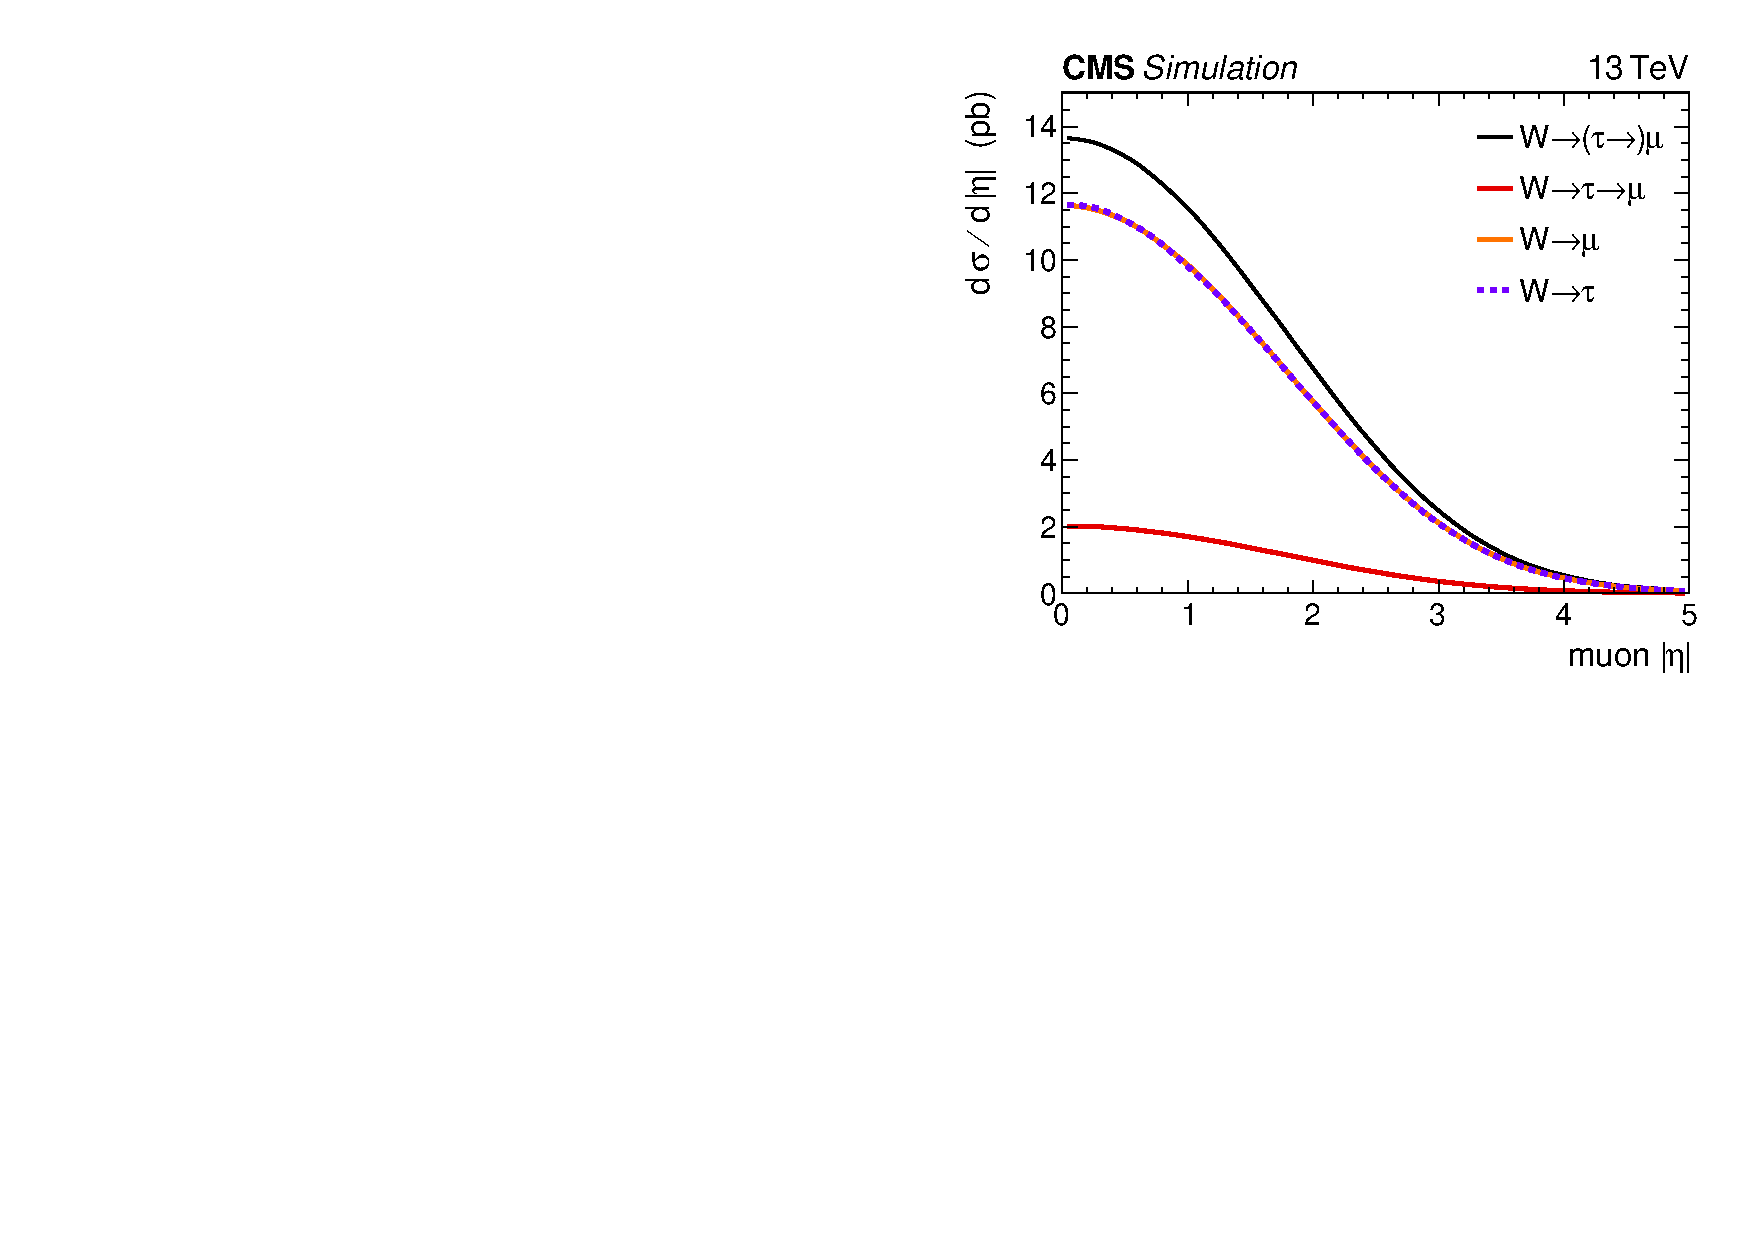
\includegraphics[width=0.48\textwidth]{figures/technique/lepton_eta.pdf}}
}
\myfigure{\label{fig:technique-parton-cosTheta}Distributions of the polarization angle for $t$-channel single top quark production at $13~\TeV$. The distributions have been generated using \POWHEG interfaced with \TAUOLA and \PYTHIA8.}{
\subfloat[]{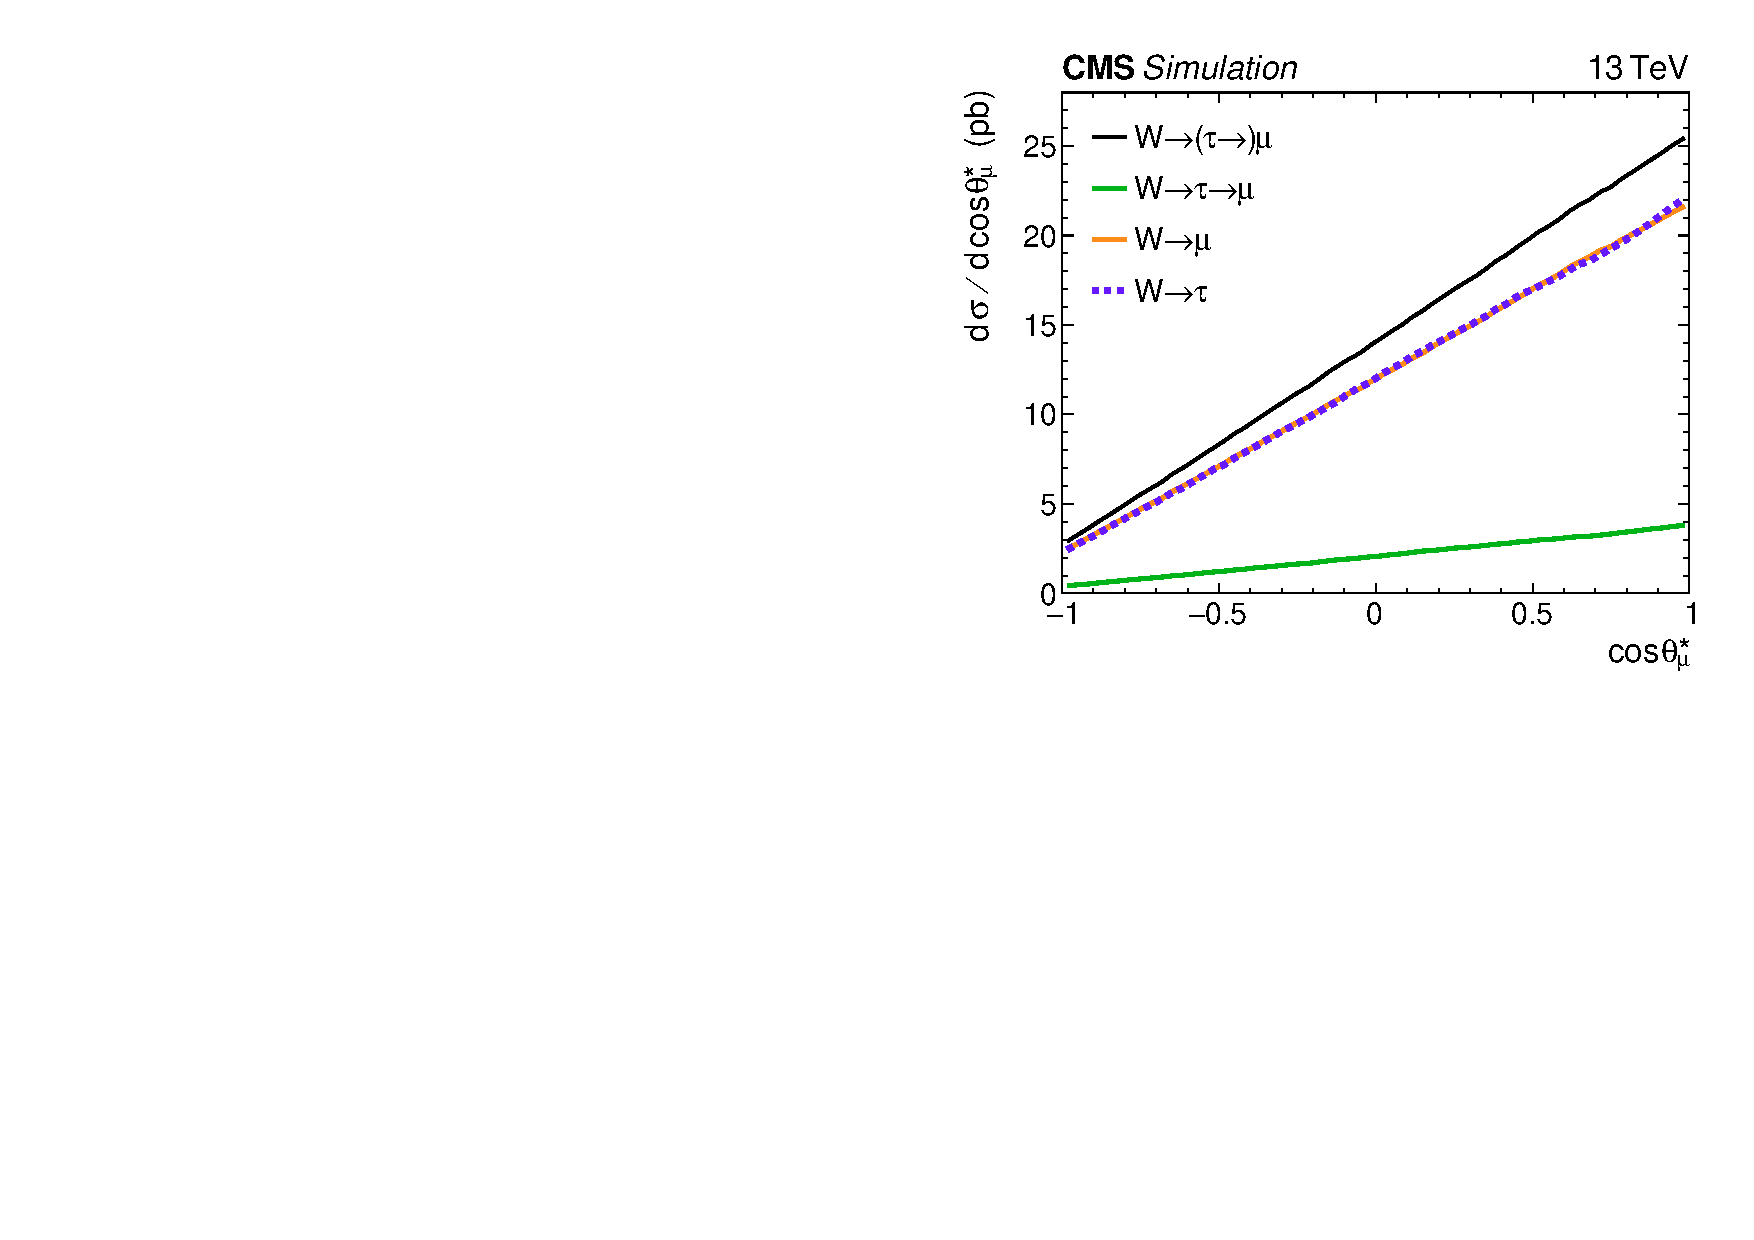
\includegraphics[width=0.48\textwidth]{figures/technique/cosTheta.pdf}}\hspace{0.03\textwidth}
\subfloat[selecting $\pt(\mu)>20~\GeV$]{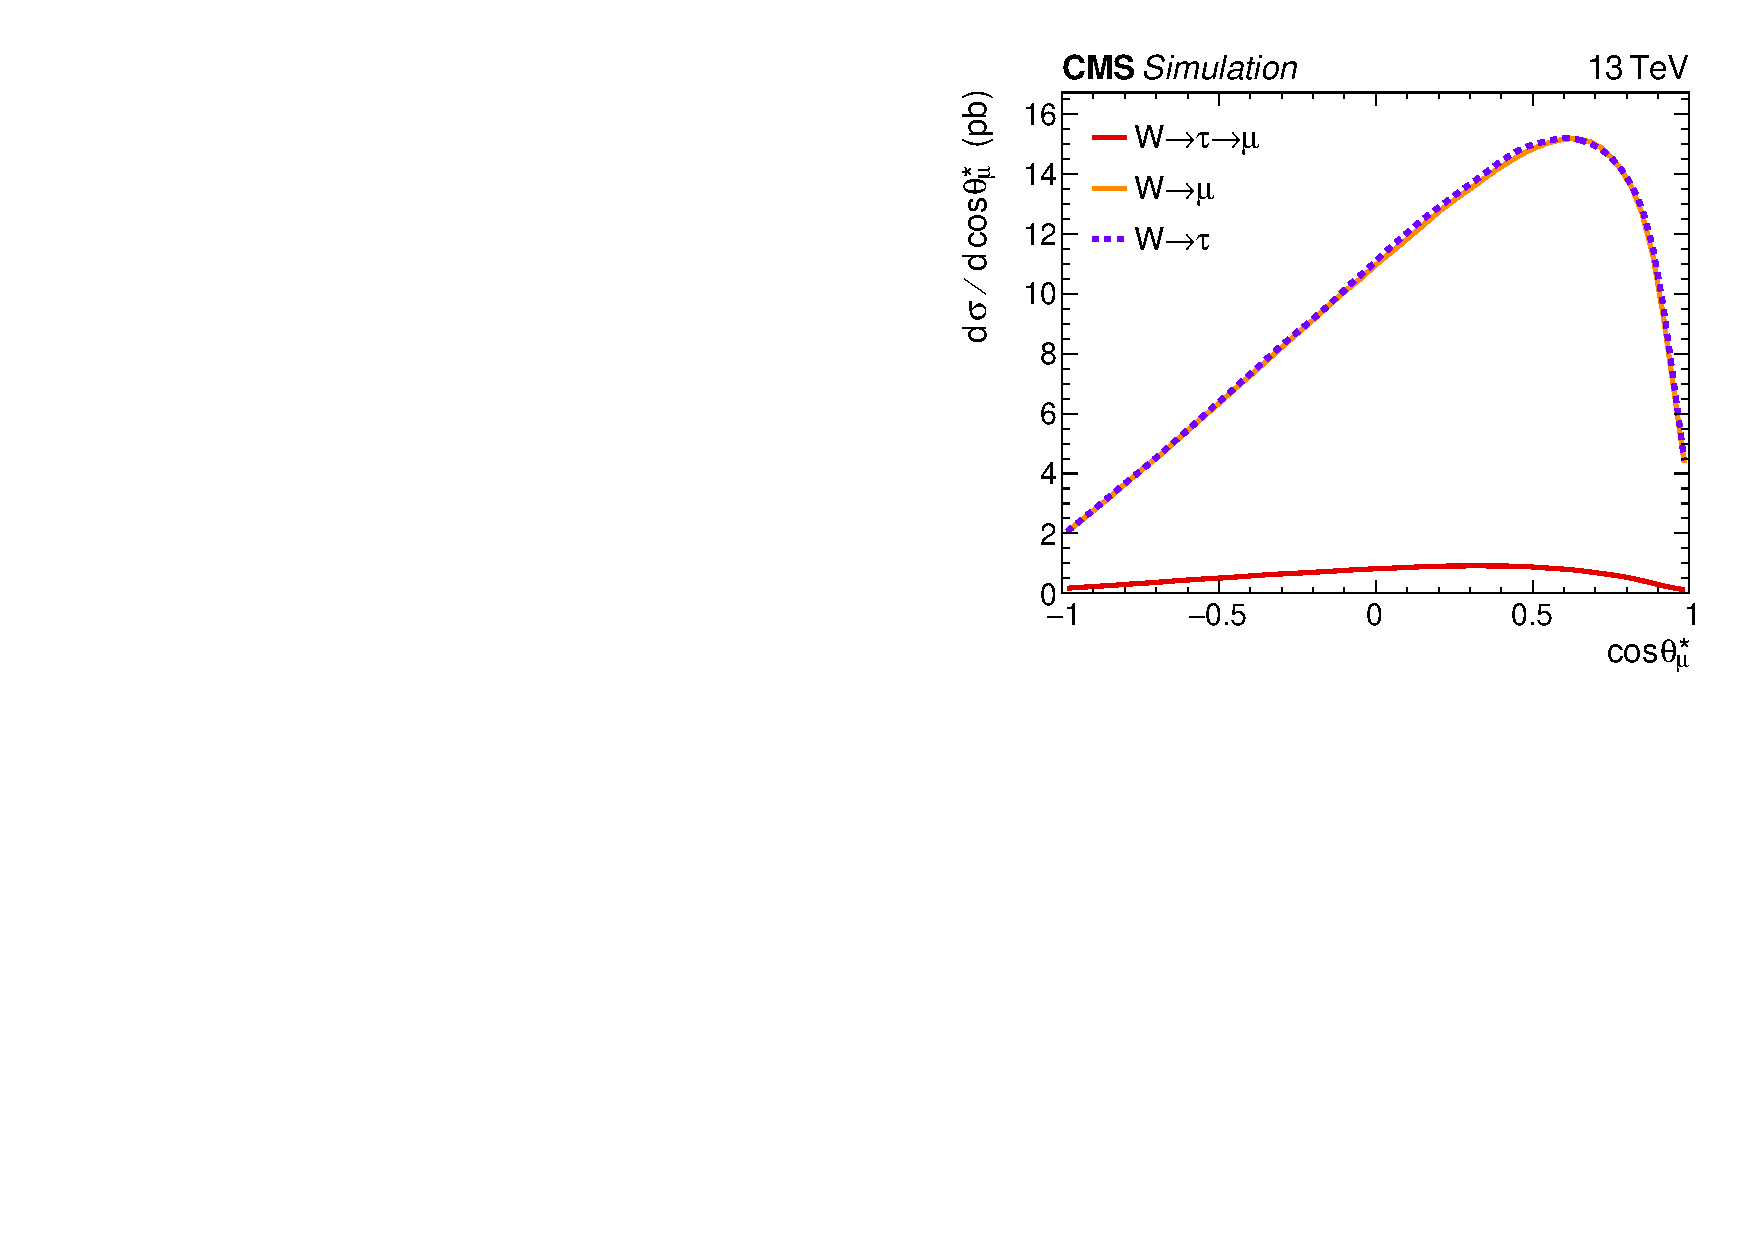
\includegraphics[width=0.48\textwidth]{figures/technique/cosTheta_lpt20.pdf}}
}

dressed leptons (cone algorithms associates photons to leptons but does not cluster close leptons), tau decays, jet clustering (no neutrinos/leptons), b-tagging, rivet, drop of cosTheta at 1 through lepton pT cut



%##############################################
\section{Unfolding}
%##############################################

Unfolding in \gls{hep} is a procedure which attempts to infer a differential cross as a function of an observable of interest at parton or particle level from data. The idea behind this is to ``revert'' the smearing effects, finite resolution and acceptance of the detector which allows to report a distribution in such a way that it can be easily compared to the expectations from theory and to potential similar measurements (even across experiments). The unfolding problem can be modeled as a Fredholm equation of the first kind

\begin{equation}
\underbrace{~f(x)~}_\mathrm{reco.}=\int \underbrace{A(x)\,\epsilon(x)\, R(x,y)}_\mathrm{detector~effects}~~\cdot \underbrace{~g(y)~}_\mathrm{parton/particle}\, \mathrm{d}y \label{eq:technique-fredholm}
\end{equation}

where $f(x)$ denotes the reconstructed distribution which is obtained by folding the true distribution $g(y)$ with the detector response $R(x,y)$ times the reconstruction efficiency $\epsilon(x)$ and the acceptance of the event selection $A(x)$. Equation~\ref{eq:technique-fredholm} can be discretized and written as matrix equation

\begin{equation}
\vec{x} = \widetilde{\mathcal{R}}\cdot\vec{y},\qquad \widetilde{\mathcal{R}}=\mathcal{A}\cdot\mathcal{E}\cdot\mathcal{R} \label{eq:technique-folding}
\end{equation}

where the continuous distributions are converted into vectors~(histograms) and the response, acceptance, and efficiency functions are described by matrices\footnote{The acceptance and efficiency are diagonal matrices.}. Elements of the response matrix $\mathcal{R}_{ij}$ can be interpreted as the transition probability $p_{i\to j}$ that an event at parton or particle level occurring in bin $i$ is measured in bin $j$. A problem occurs when solving Eq.~\ref{eq:technique-folding} for $\vec{y}$ through a simple inversion of the response matrix. Since the ?? ill-posed which leads to solutions with large variance and high anticorrelations which can be observed as oscillations~\cite{Cowan:2002in}. This problem can be understood by analyzing the unfolding problem using \glshere{svd}. It is a generalization of the eigendecomposition that allows to decompose even non-quadratic matrices into 

\begin{equation}
\vec{y}=\Big(\widetilde{\mathcal{R}}\Big)^{-1}\vec{x}\\
=\Big(\mathcal{U}~\cdot\underbrace{\mathcal{S}}_\mathrm{diagonal}\cdot~\mathcal{V}\Big)^{-1}\vec{x}~=~\mathcal{V}^{-1}\cdot\Bigg(
\begin{tikzpicture}[baseline=(current bounding box.center)]
\matrix (m) [matrix of math nodes,nodes in empty cells,row sep=-1.5mm]{
\frac{1}{s_{11}} &  & 0  \\
0 & & \frac{1}{s_{nn}} \\
} ;
\draw[dotted,thick] (m-1-1)-- (m-2-3);
\end{tikzpicture}
\Bigg)
\cdot~~\mathcal{U}^{-1}~\vec{x}
\end{equation}


where $\mathcal{U}$, $\mathcal{V}$ are the called left- and right-singular vectors respectively and $\mathcal{S}$ is a diagonal matrix whose elements $s_{ii}$ are referred to as singular values. The singular vectors can be interpreted as orthogonal modes of the measured distribution. When the singular values are small, the unfolding becomes unstable since small modes in the reconstructed distribution like statistical fluctuations can be amplified by $1/s_{ii}$ through the inversion. 

The problem can understood as following. Small bin-by-bin fluctuations of the distributions at parton/particle level are smeared out in the reconstructed distribution after folding it with the response matrix. This effect relates to small singular values which damp high order modes in the reconstructed distribution. When however an unfolding is performed of a spectrum containing such high order modes, these will receive an unphysical amplification.

Various unfolding procedures have been proposed to deal with this problem. The most straight forward regularization scheme is utilized in the \gls{svd} unfolding procedure~\cite{Hocker:1995kb} where the response matrix is modified as 

\begin{equation}
\Big(\mathcal{R}^\mathrm{reg.}[\tau]\Big)^{-1}_{ ij}=\sum_{i}^{n}\,\left(\,\sum_{k}^{\tau}~\mathcal{V}^{-1}_{ik}\cdot\left(\frac{1}{s_{kk}}\right)\cdot~\mathcal{U}^{-1}_{kj}\right).
\end{equation}

Here, the regularization parameter $\tau$ is introduced which controls a cutoff that keeps only singular values $k\leq\tau<n$ during the inversion.




to infer the 

problems, regularization scheme (thinkovo), correlations, subway plot, coverage within 2s, alternative FBU
